\section{Modelling}

\subsection{Mathematical Formulation}

The model propsed by Anderson et al. \cite{anderson_continuous_1998,anderson_mathematical_2000} 
and Chaplain et al. \cite{anderson_continuous_1998,chaplain_mathematical_2006,chaplain_mathematical_2006-1,franssen_mathematical_2019}, extended with terms for cell modelling cell proliferation consists of a system of linearly coupled partial differential equations: 

\begin{align}
	\frac{\partial c}{\partial t} &= D_c \Delta c - \chi \nabla \cdot (c\nabla e)  + \mu_1 c\left(1-\frac{c}{c_0}-\frac{e}{e_0}\right)\label{eq1}\\
	\frac{\partial e}{\partial t} &= -\delta m e  + \mu_2 c\left(1-\frac{c}{c_0}-\frac{e}{e_0}\right)\label{eq2}\\
	\frac{\partial m}{\partial t} &= D_m \Delta c + \mu_3 c - \lambda m\label{eq3}
\end{align}
with zero-flux boundary conditions, 
\begin{align}
	n\cdot (-D_c \nabla c + c \chi\nabla e) &= 0 \label{eq4}\\
	n \cdot (-D_m\nabla m ) &= 0\label{eq5}
\end{align}

where the free parameters are $D_c$, $D_m$, $\chi$, $\delta$, $\mu_1$, $\mu_2$, $\mu_3$ and $\lambda$. \newline
The variable $c$ describes the tumor cell density, $e$ the density of the extracellular matrix and $m$ the matrix-degrading enzyme concentration. All of those functions are mathematically defined to be mapping a 1,2 or 3 dimensional spacial value and a point in time to a scalar value describing the concentration at a specific point in space and time, $\{c,e,m\} : \mathbb{R}^{3} \times \mathbb{R} \rightarrow \mathbb{R}$.\newline
To derive at the expression for the tumor cell concentration $c$ we are going to assume that the tumor cell's moement is subject to two influences, haptotaxis and random movement. Haptotaxis is a directed migratory response of cells to gradients of fixed or bound chemicals \cite{anderson_continuous_1998} and random movement is influenced by for example mechanical stress, electric voltage or other such physical effects. To get an expression for how much or how fast the tumor cells move, we need to define what flux is, flux is defined to be the amount of a substance  which crosses a unit area in unit time. Incorporating the two assumed influencing factors into our mathematical model we define the haptotatic flux $J_{hapto} = \chi c \nabla e$, where $\chi$ is the haptotactic flux coefficient, and the random flux $J_{random} = -D_c \nabla c$, where $D_c$ is random mobility constant. In general this parameter could also be a function of both extracellular matrix and matrix-degrading enzyme concentration $D_c \rightarrow D(e,m)$. As we know cells proliferate and grow over time, so we want to respect this in our model with a term for tumor cell proliferation: $\mu_1 c (1-\frac{c}{c_0} - \frac{e}{e_0})$. The idea is that this term describes the cell proliferation with a logisitic growth model, $\mu_1$ describing the proliferation rate.
In the inital model proposed by Anderson et al. \cite{anderson_continuous_1998,anderson_mathematical_2000} 
and Chaplain et al. \cite{anderson_continuous_1998,chaplain_mathematical_2006,chaplain_mathematical_2006-1,franssen_mathematical_2019}, they did not respect proliferation of tumor cells and extracellular matrix and therefore applied a conservation equation for the tumor cells $\frac{\partial c}{\partial t} + \nabla \cdot (J_{hapto} + J_{random}) = 0$, in our model we extend this conservation formula with a proliferation rate. Explicitly inserting the flux formulas and logisitc growth function for the tumor cells gives us: $\frac{\partial c}{\partial t} + \nabla (J_{hapto} + J_{random}) + \mu_1 c (1-\frac{c}{c_0} - \frac{e}{e_0}) = \frac{\partial c}{\partial t} + \chi \nabla (c \nabla e) - D_c \Delta c + \mu_1 c (1-\frac{c}{c_0} - \frac{e}{e_0})$. Which is equivalent to equation \ref*{eq1}.\newline
To model the extracellular-matrix concentration $e$, we asssume that the enzymes degrade the extracellular matrix upon contact. This assumption is simply modeled by the equation $\frac{\partial e}{\partial t} = -\delta m e$, $\delta$ is a positive constant describing this annihilation process. To this we also add a term describing the proliferation process: $\frac{\partial e}{\partial t} = -\delta m e + \mu_2 c (1 - \frac{c}{c_0} - \frac{e}{e_0})$.\newline 
Modelling the matrix-degrading enzyme concentration $m$, we combine a diffusion term with production and decay terms. The diffusion term is described like in tumor cell concentration, with the addition that haptotatic fluxes are neglected and only random mobility is assumed, $J_{random} = -D_m \nabla m$. The production term depends on the tumor cell concentration and the decay term on the extracellular matrix concentration. This results in the term: $\frac{\partial m}{\partial t} = \nabla J_{random} + \mu c - \lambda e = D_m \Delta m + \mu_3 c - \lambda m$, $\mu$ and $\delta$ describing production and decay rates.


\subsection{Numerical Model and Parameters}

To make solving the model easier we are first going to non-dimensionalise all the equations \ref*{eq1} - \ref*{eq5} in a standard way, with the goal to rescale the space domain onto unit size. For one space dimension this results in the unit interval $[0,1]$, for two dimensions the unit square $[0,1] \times [0,1]$ and for three dimensions the unit cube $[0,1] \times [0,1] \times [0,1]$. 
We start with rescaling the distance with an appropriate length scale $L$ and the time with $\tau = \frac{L^2}{D}$ ($D$ being a chemical diffusion coefficient). The three variables are being rescaled with their initial values respectively $c_0, e_0, m_0$, which gives us this:
\begin{align}
    \tilde{c} = \frac{c}{c_0};  \tilde{e} = \frac{e}{e_0};  \tilde{m} = \frac{m}{m_0}  
\end{align}

Next we modify the system's free parameters $D_c, \chi, \delta, D_m, \mu_3, \lambda$: \newline 
\begin{center}
    $d_c = \frac{D_c}{D},\quad \gamma = \chi \frac{e_0}{D},\quad \eta = \tau m_0 \delta,\quad d_m = \frac{D_m}{D},\quad \alpha = \tau \mu_3 \frac{c_0}{m_0},\quad \beta = \tau \lambda$.
\end{center} 
with $D$ being a refrence chemical diffusion coeffizcient.\newline 
These modifications make the new system of linearly coupled partial differential equations, where the tildes are dropped for simplicitie's sake:
\begin{align}
	\frac{\partial c}{\partial t} &= d_c \Delta c - \gamma \nabla \cdot (c\nabla e)  + \mu_1 c\left(1-\frac{c}{c_0}-\frac{e}{e_0}\right)\\
	\frac{\partial e}{\partial t} &= -\eta m e  + \mu_2 c\left(1-\frac{c}{c_0}-\frac{e}{e_0}\right)\\
	\frac{\partial m}{\partial t} &= d_m \Delta c + \alpha c - \beta m
\end{align}
with also updated zero-flux boundary conditions, 
\begin{align}
	\zeta \cdot (-d_c \nabla c + c \gamma \nabla e) &= 0\\
	\zeta \cdot (-d_m\nabla m ) &= 0
\end{align}
where $\zeta$ is an appropriate outward unit normal vector.\newline 
In order to use the finite element method we will change to the variational formulation. If we assume each species to be in the Hilbert space $H^1(\Omega)$, the variational formulation can be derived by multiplying with a test function, integrating over the domain $\Omega$ and use integration by parts and the Gauss theorem. This will give us a broader solution space and reduces the requirements of the solution regarding differentiability. With $\left(\cdot, \cdot\right)$ denoting the $L^2$-scalar product on $\Omega$ the following equation system results

\begin{align}
    \left(\frac{\partial c}{\partial t}, \varphi_c\right) &=
        - D_c\left(\nabla c, \nabla \varphi_c\right) + \chi \left(c\nabla e, \nabla \varphi_c\right) + \mu_1 \left(c \cdot \left(1-\frac{c}{c_0} - \frac{e}{e_0}\right), \varphi_c\right)     \\
    \left(\frac{\partial e}{\partial t}, \varphi_e\right) &=  -\delta \left( me, \varphi_e\right) + \mu_2 \left(e\left(1-\frac{c}{c_0}-\frac{e}{e_0}\right),\varphi_e\right) \\
    \left(\frac{\partial m}{\partial t}, \varphi_m\right) &= -D_m \left(\nabla m,\nabla \varphi_m\right) + \mu_e \left(c,\varphi_m\right) - \lambda \left(m,\varphi_m\right) 
\end{align}

For the initial conditions we will assume that at dimensionless time $\tau = 0$, there is already a nodule of cells present centered around the origin in every dimension. For example in one dimension $c$ is having the initial density distribution,
$c(x,0)=
\begin{cases}
exp(\frac{-x^2}{\epsilon}), x\in [-0.25, 0.25]\\
0, x\notin [-0.25,0.25]
\end{cases}
$, with $\epsilon$ being a postive constant. 
The tumor will have degraded some of its surrounding tissue in every experiment and hence we take the inital profile of the extracellular matrix to be $e(x,0) = 1 - 0.5 c(x,0)$. At last we assume the initial matrix-degrading enzyme concentration to be proportional to the initial tumor cell density and therefore take $m(x,0) = 0.5 c(x,0)$. These inital values are displayed in figure \ref{fig:Initial_Value_Distribution}.
\begin{figure}
    \centering
    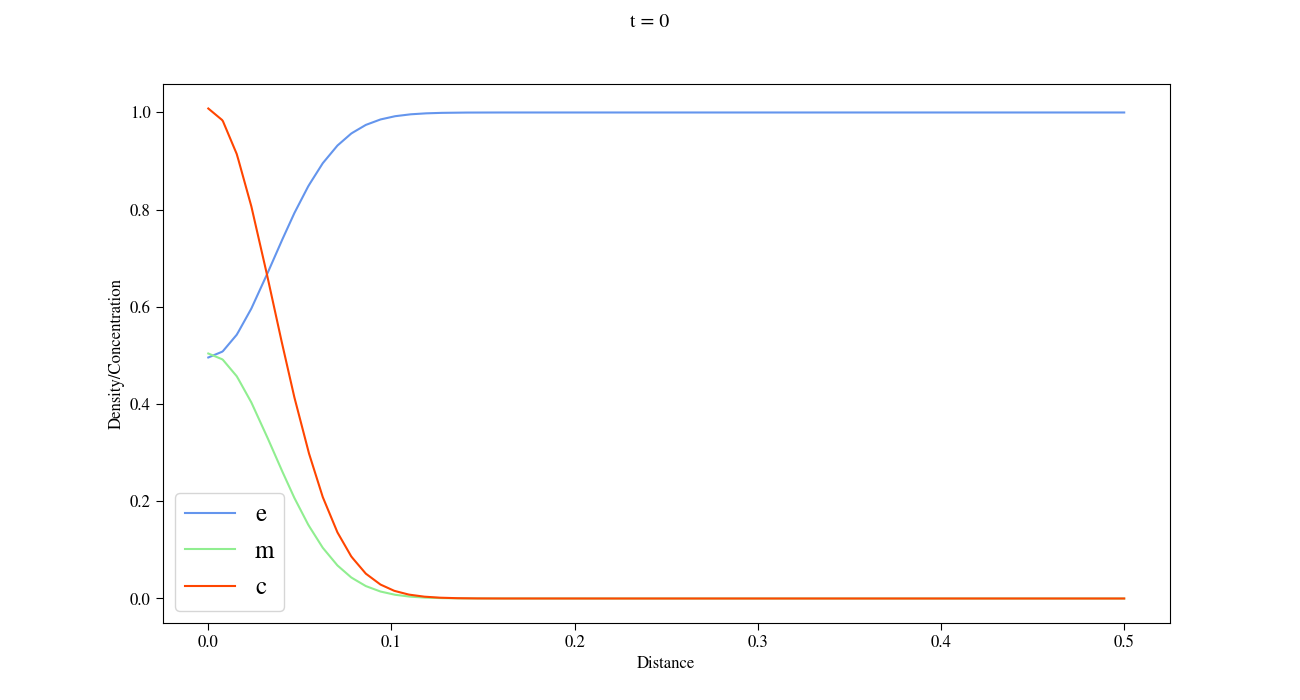
\includegraphics[width=\textwidth]{resources/images/inital_value_plot_figure.png}
    \caption{Visualization of the initial value distribution for an experiment in two space dimensions, radially symmetrical}
    \label{fig:Initial_Value_Distribution}
\end{figure}

For each of the modified free parameters $d_c, \gamma, \eta, d_m, \alpha, \beta, \mu_1, \mu_2$ we are going to take look at values or ranges which were used in previous experiments: 
\begin{itemize}
    \item $d_c = 0.001$
    \item $\gamma \in \{0.001, 0.002, 0.005\}$
    \item $\mu_1 \in \{0.1, 0.5\}$
    \item $\eta \in \{10, 20\}$
    \item $\mu_2 \in \{0.1, 0.5\}$
    \item $d_m \in \{0.001, 0.01\}$
    \item $\alpha \in \{0.1, 10\}$
    \item $\beta \in \{0, 0.07, 0.5\}$
\end{itemize}








\begin{comment}
For each of the above parameters we are going to look reasonable ranges in which they are definded:
\begin{itemize}
    \item $D_c$: As explained it is cruical for tumor cells to have a high motility, evading the defense mechanisms of cells and invading surrouding tissue effectively. 
    The diffusion coefficient $D_c$ ranges with values ranging from ... to ...
    \item $D_m$: Since an extracellular matrix describes a network of extracellular macromolecules and minerals, it's diffusion properties heavily depend 
    on the components this network is build of, they can be for example be collagens or enzymes that provide structural and 
    biochemical support for the surrouding cells. This causes the coefficient to vary widely with a range of ... to .....
    \item $\chi$: The parameter $\chi$ describes movement responses of tumor cells to changes in attracting molecules concentration, like in our case the 
    extracellular matrix concentration. The parameter's range lies between ... and ....
    \item $\delta$: $\delta$ models the annihilation process of matrix-degrading enzymes and extracellular matrix macromolecules.
    It has usually a value between .. and ..
    \item $\mu_i$: The value of $\mu_i$ will respectively describe the production rate of tumor cells, extracellular matrix macromolecules and matrix-degrading enzymes, for $i\in \{1,2,3\}$.
    
    \item $\lambda$: This parameter describes the production rate of the matrix-degrading enzymes. Here we have values within the range ... to ...
\end{itemize}
These ranges will later govern the parameter analysis in the Experiment section.

\subsubsection{Diffusion Koefficient $D_x$}
Those parameters are now given an in-depth biological meaning and assumptions on their areas of definition. \newline 
Starting with $D_c$ and $D_m$, they are the diffusion coefficients, describing how fast a particle may diffuse through a medium. 
Diffusion means particles moving from areas of higher concentration to areas of lower concentration, with the goal of creating an equillibrium 
state, where everywhere of the defined space we have the same concentration of particles. For example knwoing from the biological foundation 
that cancer cells need to have a higher motility than normal cells to invade the surrouding tissue, the diffusion coefficients for 
the malignant cells is likely to be higher than the one of normal cells. 
In mathematical terms Fick's Law is often used to describe diffusion, creating a relationship between a concentration gradient and the flux of a substance. 
The flux describes the amount of a substances which crosses a unit area in unit time:
\begin{align}
    F = - D \frac{\partial c}{\partial x} = -D \nabla c
\end{align}
With this formulation 

\subsubsection{Haptotatic Flux Koefficient}
$\chi$

\subsubsection{Production and Decay Rates}
$\lambda$, $mu$


\subsubsection{Degradation}
$\delta$

\subsubsection{Assumptions}
\end{comment}